%!TEX program = xelatex
\RequirePackage{xr-hyper}
\documentclass[lang=cn,a4paper,newtx]{elegantpaper}
\title{阈值策略下接触控制与追踪隔离的最优控制：补充材料}
\author{XXX \and XXX}
\institute{School of Mathematics and Statistics, Shaanxi Normal University}
\date{}
\usepackage{amsmath,amssymb,array,tabularx,makecell,threeparttable,siunitx,xurl,graphicx,float,placeins,multirow,needspace,xr-hyper}
\externaldocument{flatten_curve_analysis_cn}
\graphicspath{{./}{figures/}{table/}}
\numberwithin{equation}{section}
\theoremstyle{plain}
\newtheorem{corollaryn}[theorem]{推论}
\newtheorem{remarkn}[theorem]{注记}
\allowdisplaybreaks[3]
\newcommand{\qinf}{q_{\mathrm{inf}}}
\newcommand{\Itcum}{I_{t_{\mathrm{cum}}}}
% 由 nr_audit/make_numbers.py 生成，勿手改。字段映射见 nr_audit/results/nr_numbers_map.json。
% 含 \times 的宏须在数学模式中使用。
\newcommand{\nrICtOneLow}{18.48}  % 西安（η = 0.001N）仅隔离控制的启动时刻 t1，I0 为拟合值的 0.1 倍
\newcommand{\nrICtOneFit}{16.20}  % 西安（η = 0.001N）仅隔离控制的启动时刻 t1，I0 为拟合值的 1 倍
\newcommand{\nrICtOneHigh}{13.93}  % 西安（η = 0.001N）仅隔离控制的启动时刻 t1，I0 为拟合值的 10 倍
\newcommand{\nrICtOneShift}{2.28}  % I0 改为 0.1 或 10 倍时 t1 的最大变化（η = 0.001N，两种控制相同）
\newcommand{\nrICMaxRelSstar}{3.1\times10^{-9}}  % 六条轨迹中 S_star 相对拟合初值的最大相对变化（η = 0.001N）
\newcommand{\nrICMaxRelDt}{1.6\times10^{-9}}  % 六条轨迹中 dt 相对拟合初值的最大相对变化（η = 0.001N）
\newcommand{\nrICMaxRelJ}{4.3\times10^{-9}}  % 六条轨迹中 J 相对拟合初值的最大相对变化（η = 0.001N）
\newcommand{\nrICMaxRelTotal}{4.5\times10^{-9}}  % 六条轨迹中 total_infections_to_clearance 相对拟合初值的最大相对变化（η = 0.001N）
\newcommand{\nrICtabQLowTOne}{18.48}  % 西安（η = 0.001N）固定人口初值诊断：q_only，I0 为拟合值的 0.1 倍，t1
\newcommand{\nrICtabQLowDt}{170.6301}  % 西安（η = 0.001N）固定人口初值诊断：q_only，I0 为拟合值的 0.1 倍，dt
\newcommand{\nrICtabQLowJ}{82.119}  % 西安（η = 0.001N）固定人口初值诊断：q_only，I0 为拟合值的 0.1 倍，J
\newcommand{\nrICtabQLowTend}{391.59}  % 西安（η = 0.001N）固定人口初值诊断：q_only，I0 为拟合值的 0.1 倍，t_end
\newcommand{\nrICtabQFitTOne}{16.20}  % 西安（η = 0.001N）固定人口初值诊断：q_only，I0 为拟合值的 1 倍，t1
\newcommand{\nrICtabQFitDt}{170.6301}  % 西安（η = 0.001N）固定人口初值诊断：q_only，I0 为拟合值的 1 倍，dt
\newcommand{\nrICtabQFitJ}{82.119}  % 西安（η = 0.001N）固定人口初值诊断：q_only，I0 为拟合值的 1 倍，J
\newcommand{\nrICtabQFitTend}{389.32}  % 西安（η = 0.001N）固定人口初值诊断：q_only，I0 为拟合值的 1 倍，t_end
\newcommand{\nrICtabQHighTOne}{13.93}  % 西安（η = 0.001N）固定人口初值诊断：q_only，I0 为拟合值的 10 倍，t1
\newcommand{\nrICtabQHighDt}{170.6301}  % 西安（η = 0.001N）固定人口初值诊断：q_only，I0 为拟合值的 10 倍，dt
\newcommand{\nrICtabQHighJ}{82.119}  % 西安（η = 0.001N）固定人口初值诊断：q_only，I0 为拟合值的 10 倍，J
\newcommand{\nrICtabQHighTend}{387.04}  % 西安（η = 0.001N）固定人口初值诊断：q_only，I0 为拟合值的 10 倍，t_end
\newcommand{\nrICtabOLowTOne}{18.48}  % 西安（η = 0.001N）固定人口初值诊断：opt，I0 为拟合值的 0.1 倍，t1
\newcommand{\nrICtabOLowDt}{218.1027}  % 西安（η = 0.001N）固定人口初值诊断：opt，I0 为拟合值的 0.1 倍，dt
\newcommand{\nrICtabOLowJ}{76.624}  % 西安（η = 0.001N）固定人口初值诊断：opt，I0 为拟合值的 0.1 倍，J
\newcommand{\nrICtabOLowTend}{439.07}  % 西安（η = 0.001N）固定人口初值诊断：opt，I0 为拟合值的 0.1 倍，t_end
\newcommand{\nrICtabOFitTOne}{16.20}  % 西安（η = 0.001N）固定人口初值诊断：opt，I0 为拟合值的 1 倍，t1
\newcommand{\nrICtabOFitDt}{218.1027}  % 西安（η = 0.001N）固定人口初值诊断：opt，I0 为拟合值的 1 倍，dt
\newcommand{\nrICtabOFitJ}{76.624}  % 西安（η = 0.001N）固定人口初值诊断：opt，I0 为拟合值的 1 倍，J
\newcommand{\nrICtabOFitTend}{436.79}  % 西安（η = 0.001N）固定人口初值诊断：opt，I0 为拟合值的 1 倍，t_end
\newcommand{\nrICtabOHighTOne}{13.93}  % 西安（η = 0.001N）固定人口初值诊断：opt，I0 为拟合值的 10 倍，t1
\newcommand{\nrICtabOHighDt}{218.1027}  % 西安（η = 0.001N）固定人口初值诊断：opt，I0 为拟合值的 10 倍，dt
\newcommand{\nrICtabOHighJ}{76.624}  % 西安（η = 0.001N）固定人口初值诊断：opt，I0 为拟合值的 10 倍，J
\newcommand{\nrICtabOHighTend}{434.51}  % 西安（η = 0.001N）固定人口初值诊断：opt，I0 为拟合值的 10 倍，t_end
\newcommand{\nrFitMseCommNew}{47.33}  % 拟合初值下 community_new 的均方误差
\newcommand{\nrFitMseQuarNew}{130.38}  % 拟合初值下 quarantine_new 的均方误差
\newcommand{\nrFitMseCommCum}{387.22}  % 拟合初值下 community_cum 的均方误差
\newcommand{\nrFitMseQuarCum}{471.84}  % 拟合初值下 quarantine_cum 的均方误差
\newcommand{\nrFitObjective}{1036.76}  % 四项均方误差之和（拟合准则）
\newcommand{\nrWtBaseAToApLo}{3.1354}  % base：结构由 A 变为 A' 的 r 括区下端（宽度 < 1e-3，所检验网格上）
\newcommand{\nrWtBaseAToApHi}{3.1361}  % base：结构由 A 变为 A' 的 r 括区上端（宽度 < 1e-3，所检验网格上）
\newcommand{\nrWtBaseAToApApx}{3.14}  % base：结构由 A 变为 A' 的 r 括区中点取两位小数（正文用语“约”，不是括区端点）
\newcommand{\nrWtBaseApToBLo}{3.2050}  % base：结构由 A' 变为 B 的 r 括区下端（宽度 < 1e-3，所检验网格上）
\newcommand{\nrWtBaseApToBHi}{3.2057}  % base：结构由 A' 变为 B 的 r 括区上端（宽度 < 1e-3，所检验网格上）
\newcommand{\nrWtBaseApToBApx}{3.21}  % base：结构由 A' 变为 B 的 r 括区中点取两位小数（正文用语“约”，不是括区端点）
\newcommand{\nrWtBaseBToCLo}{13.1011}  % base：结构由 B 变为 C 的 r 括区下端（宽度 < 1e-3，所检验网格上）
\newcommand{\nrWtBaseBToCHi}{13.1018}  % base：结构由 B 变为 C 的 r 括区上端（宽度 < 1e-3，所检验网格上）
\newcommand{\nrWtBaseBToCApx}{13.10}  % base：结构由 B 变为 C 的 r 括区中点取两位小数（正文用语“约”，不是括区端点）
\newcommand{\nrWtXianAToApLo}{2.5477}  % xian：结构由 A 变为 A' 的 r 括区下端（宽度 < 1e-3，所检验网格上）
\newcommand{\nrWtXianAToApHi}{2.5482}  % xian：结构由 A 变为 A' 的 r 括区上端（宽度 < 1e-3，所检验网格上）
\newcommand{\nrWtXianAToApApx}{2.55}  % xian：结构由 A 变为 A' 的 r 括区中点取两位小数（正文用语“约”，不是括区端点）
\newcommand{\nrWtXianApToBLo}{2.7086}  % xian：结构由 A' 变为 B 的 r 括区下端（宽度 < 1e-3，所检验网格上）
\newcommand{\nrWtXianApToBHi}{2.7092}  % xian：结构由 A' 变为 B 的 r 括区上端（宽度 < 1e-3，所检验网格上）
\newcommand{\nrWtXianApToBApx}{2.71}  % xian：结构由 A' 变为 B 的 r 括区中点取两位小数（正文用语“约”，不是括区端点）
\newcommand{\nrWtXianBToCLo}{7.5108}  % xian（η = 0.001N）：结构由 B 变为 C 的 r 括区下端（宽度 < 1e-3）
\newcommand{\nrWtXianBToCHi}{7.5118}  % xian（η = 0.001N）：结构由 B 变为 C 的 r 括区上端（宽度 < 1e-3）
\newcommand{\nrWtXianBToCApx}{7.51}  % xian（η = 0.001N）：结构由 B 变为 C 的 r 括区中点取两位小数（正文用语“约”）
\newcommand{\nrConvTolMaxRel}{3\times10^{-12}}  % 积分容差三档间核心量的最大相对变化（阈值策略的全部轨迹）
\newcommand{\nrConvNzMaxRel}{1\times10^{-13}}  % N_z = 4001 与 8001 的 Δt、J 最大相对差
\newcommand{\nrConvNxMaxGap}{1\times10^{-13}}  % 控制网格上网格值低于根法值的最大相对量
\newcommand{\nrPlateauDevBase}{2.1\times10^{-11}}  % base 仅隔离控制开环完整方程阈值控制期的 max|I-η|（基准档）
\newcommand{\nrPlateauDevXian}{6.9\times10^{-11}}  % xian 仅隔离控制开环完整方程阈值控制期的 max|I-η|（基准档）
\newcommand{\nrConvNzAllMaxRel}{7.3\times10^{-13}}  % N_z = 1001、2001、4001 与 8001 的 Δt、J 最大相对差
\newcommand{\nrConvNzQuadMaxRel}{2.0\times10^{-13}}  % N_z = 8001 的 Simpson 与分段 quad 的 Δt、J 最大相对差
\newcommand{\nrConvPlateauMax}{4.6\times10^{-9}}  % 积分容差三档下阈值控制期 max|I-η| 的最大值
\newcommand{\nrConvExitMax}{1.8\times10^{-7}}  % 积分容差三档下退出时刻 S 与 S_c 之差的最大值
\newcommand{\nrConvMassMax}{1.3\times10^{-6}}  % 积分容差三档下人口守恒残差的最大值（含常规控制与 TDINN）
\newcommand{\nrTdinnTolChange}{1.5\times10^{-11}}  % 本模块收紧容差并把最大步长减半后，TDINN 总累计新增感染（清零时间）的变化
\newcommand{\nrIdentityMaxRel}{4\times10^{-14}}  % 累计新增感染恒等式残差/初始易感者总数的最大值
\newcommand{\nrRetLBase}{586.84}  % base：L = U(0) − S_c = S_0 + S_q(0) − S_c
\newcommand{\nrRetCinfBaseQ}{286.59}  % base：无回流（ω=0）q_only 的 t→∞ 累计新增感染 C_π(0)
\newcommand{\nrRetClrBaseQ}{285.7}  % base：无回流 q_only 计至清零时间的累计新增感染（表 2）
\newcommand{\nrRetCinfBaseA}{324.25}  % base：无回流（ω=0）alpha 的 t→∞ 累计新增感染 C_π(0)
\newcommand{\nrRetCinfBaseO}{307.50}  % base：无回流（ω=0）opt 的 t→∞ 累计新增感染 C_π(0)
\newcommand{\nrRetClrBaseO}{306.6}  % base：无回流 opt 计至清零时间的累计新增感染（表 2）
\newcommand{\nrRetCinfBaseC}{629.51}  % base：无回流（ω=0）c_only 的 t→∞ 累计新增感染 C_π(0)
\newcommand{\nrRetClrBaseC}{628.6}  % base：无回流 c_only 计至清零时间的累计新增感染（表 2）
\newcommand{\nrRetLXian}{10.1889}  % xian：L = U(0) − S_c = S_0 + S_q(0) − S_c
\newcommand{\nrRetCinfXianQ}{2.3779}  % xian：无回流（ω=0）q_only 的 t→∞ 累计新增感染 C_π(0)
\newcommand{\nrRetClrXianQ}{2.3779}  % xian：无回流 q_only 计至清零时间的累计新增感染（表 2）
\newcommand{\nrRetCinfXianA}{2.6390}  % xian：无回流（ω=0）alpha 的 t→∞ 累计新增感染 C_π(0)
\newcommand{\nrRetCinfXianO}{2.5348}  % xian：无回流（ω=0）opt 的 t→∞ 累计新增感染 C_π(0)
\newcommand{\nrRetClrXianO}{2.5348}  % xian：无回流 opt 计至清零时间的累计新增感染（表 2）
\newcommand{\nrRetCinfXianC}{3.8566}  % xian：无回流（ω=0）c_only 的 t→∞ 累计新增感染 C_π(0)
\newcommand{\nrRetClrXianC}{3.8566}  % xian：无回流 c_only 计至清零时间的累计新增感染（表 2）
\newcommand{\nrRetTermBaseSevenQ}{655.35}  % base：指数回流 1/ω=7 d，q_only，终止时（退出后首次 I<1）累计新增感染；来源见 source
\newcommand{\nrRetTermBaseSevenM}{657.51}  % base：指数回流 1/ω=7 d，opt_noreturn，终止时（退出后首次 I<1）累计新增感染；来源见 source
\newcommand{\nrRetTermBaseSevenC}{672.53}  % base：指数回流 1/ω=7 d，c_only，终止时（退出后首次 I<1）累计新增感染；来源见 source
\newcommand{\nrRetTermBaseFourteenQ}{619.48}  % base：指数回流 1/ω=14 d，q_only，终止时（退出后首次 I<1）累计新增感染；来源见 source
\newcommand{\nrRetTermBaseFourteenM}{620.50}  % base：指数回流 1/ω=14 d，opt_noreturn，终止时（退出后首次 I<1）累计新增感染；来源见 source
\newcommand{\nrRetTermBaseFourteenC}{665.80}  % base：指数回流 1/ω=14 d，c_only，终止时（退出后首次 I<1）累计新增感染；来源见 source
\newcommand{\nrRetTermBaseThirtyQ}{594.44}  % base：指数回流 1/ω=30 d，q_only，终止时（退出后首次 I<1）累计新增感染；来源见 source
\newcommand{\nrRetTermBaseThirtyM}{595.90}  % base：指数回流 1/ω=30 d，opt_noreturn，终止时（退出后首次 I<1）累计新增感染；来源见 source
\newcommand{\nrRetTermBaseThirtyC}{654.44}  % base：指数回流 1/ω=30 d，c_only，终止时（退出后首次 I<1）累计新增感染；来源见 source
\newcommand{\nrRetTermXianSevenQ}{10.5485}  % xian：指数回流 1/ω=7 d，q_only，终止时（退出后首次 I<1）累计新增感染；来源见 source
\newcommand{\nrRetTermXianSevenM}{10.5491}  % xian：指数回流 1/ω=7 d，opt_noreturn，终止时（退出后首次 I<1）累计新增感染；来源见 source
\newcommand{\nrRetTermXianSevenC}{10.5495}  % xian：指数回流 1/ω=7 d，c_only，终止时（退出后首次 I<1）累计新增感染；来源见 source
\newcommand{\nrRetTermXianFourteenQ}{10.4498}  % xian：指数回流 1/ω=14 d，q_only，终止时（退出后首次 I<1）累计新增感染；来源见 source
\newcommand{\nrRetTermXianFourteenM}{10.4520}  % xian：指数回流 1/ω=14 d，opt_noreturn，终止时（退出后首次 I<1）累计新增感染；来源见 source
\newcommand{\nrRetTermXianFourteenC}{10.4538}  % xian：指数回流 1/ω=14 d，c_only，终止时（退出后首次 I<1）累计新增感染；来源见 source
\newcommand{\nrRetTermXianThirtyQ}{10.3044}  % xian：指数回流 1/ω=30 d，q_only，终止时（退出后首次 I<1）累计新增感染；来源见 source
\newcommand{\nrRetTermXianThirtyM}{10.3031}  % xian：指数回流 1/ω=30 d，opt_noreturn，终止时（退出后首次 I<1）累计新增感染；来源见 source
\newcommand{\nrRetTermXianThirtyC}{10.3018}  % xian：指数回流 1/ω=30 d，c_only，终止时（退出后首次 I<1）累计新增感染；来源见 source
\newcommand{\nrRetTailBaseSeven}{1.581}  % base：平均停留7d三控制的最大剩余感染上界，显示向上取整
\newcommand{\nrRetTailBaseFourteen}{4.435}  % base：平均停留14d三控制的最大剩余感染上界，显示向上取整
\newcommand{\nrRetTailBaseThirty}{22.374}  % base：平均停留30d三控制的最大剩余感染上界，显示向上取整
\newcommand{\nrRetTailXianSeven}{10.738}  % xian：平均停留7d三控制的最大剩余感染上界，显示向上取整
\newcommand{\nrRetTailXianFourteen}{15.359}  % xian：平均停留14d三控制的最大剩余感染上界，显示向上取整
\newcommand{\nrRetTailXianThirty}{37.440}  % xian：平均停留30d三控制的最大剩余感染上界，显示向上取整
\newcommand{\nrRetSolverTolRel}{2.6\times10^{-11}}  % 固定来源54条容差对照中收紧后的核心量最大相对变化
\newcommand{\nrCostRcontBase}{3.1358}  % base：连续结构定理的权重界 r_cont(b) = 16/(b+sqrt(b^2-8b+8))^2
\newcommand{\nrCostRhatBase}{3.2051}  % base：前段仅隔离控制全局最优的权重界 r̂(b) = (S_sw/(S_sw-S_c))^2
\newcommand{\nrCostGapOneBase}{2.3}  % base：r = 1 时 100(1 - J_min/J_q-only)，即成本最优控制比仅隔离控制低的百分比
\newcommand{\nrCostRcontXian}{2.5477}  % xian：连续结构定理的权重界 r_cont(b) = 16/(b+sqrt(b^2-8b+8))^2
\newcommand{\nrCostRhatXian}{2.7090}  % xian：前段仅隔离控制全局最优的权重界 r̂(b) = (S_sw/(S_sw-S_c))^2
\newcommand{\nrCostGapOneXian}{3.0}  % xian（η = 0.001N）：r = 1 时 100(1 - J_min/J_q-only)
\newcommand{\nrRwBaseQDt}{19.21}  % base，1/ω = 14 d：仅隔离控制的控制时长
\newcommand{\nrRwBaseQJ}{2.823}  % base，1/ω = 14 d：仅隔离控制的成本 J（w_c = 1、w_q = 2）
\newcommand{\nrRwBaseQInf}{619.48}  % base，1/ω = 14 d：仅隔离控制计至 T_cut 的累计新增感染
\newcommand{\nrRwBaseODt}{20.69}  % base，1/ω = 14 d：回流下的成本最优控制的控制时长
\newcommand{\nrRwBaseOJ}{2.765}  % base，1/ω = 14 d：回流下的成本最优控制的成本 J（w_c = 1、w_q = 2）
\newcommand{\nrRwBaseOInf}{619.90}  % base，1/ω = 14 d：回流下的成本最优控制计至 T_cut 的累计新增感染
\newcommand{\nrRwBaseMDt}{21.81}  % base，1/ω = 14 d：无回流成本最优律的控制时长
\newcommand{\nrRwBaseMJ}{2.842}  % base，1/ω = 14 d：无回流成本最优律的成本 J（w_c = 1、w_q = 2）
\newcommand{\nrRwBaseMInf}{620.50}  % base，1/ω = 14 d：无回流成本最优律计至 T_cut 的累计新增感染
\newcommand{\nrRwBaseCDt}{38.47}  % base，1/ω = 14 d：仅减少接触的控制时长
\newcommand{\nrRwBaseCJ}{12.579}  % base，1/ω = 14 d：仅减少接触的成本 J（w_c = 1、w_q = 2）
\newcommand{\nrRwBaseCInf}{665.80}  % base，1/ω = 14 d：仅减少接触计至 T_cut 的累计新增感染
\newcommand{\nrRwBaseFrontPct}{11}  % base：回流下成本最优控制 λ 首次低于 0.99 的控制期比例（仅隔离前段）
\newcommand{\nrRwBaseMigGapPct}{2.8}  % base：沿用无回流成本最优律比回流下最低成本高出的百分比
\newcommand{\nrRwBaseL}{587}  % base：U(0) - S_c
\newcommand{\nrRwBaseDiffPct}{7.5}  % base，1/ω = 14 d：仅减少接触比仅隔离控制多出的累计感染（%）
\newcommand{\nrRwBaseDiffPctNoret}{120}  % base，无回流：仅减少接触比仅隔离控制多出的累计感染（%，计至清零）
\newcommand{\nrRwBaseQDtNoret}{5.90}  % base，无回流：仅隔离控制的控制时长
\newcommand{\nrRwBaseUMin}{0.55}  % base：各轨迹终止时 (S+S_q)/S_c 的最小值
\newcommand{\nrRwBaseUMax}{0.81}  % base：各轨迹终止时 (S+S_q)/S_c 的最大值
\newcommand{\nrRwXianQDt}{815.3}  % xian，1/ω = 14 d：仅隔离控制的控制时长
\newcommand{\nrRwXianQJ}{409.39}  % xian，1/ω = 14 d：仅隔离控制的成本 J（w_c = 1、w_q = 2）
\newcommand{\nrRwXianQInf}{10.4172}  % xian，1/ω = 14 d：仅隔离控制计至 T_cut 的累计新增感染
\newcommand{\nrRwXianODt}{1002.9}  % xian，1/ω = 14 d：回流下的成本最优控制的控制时长
\newcommand{\nrRwXianOJ}{369.24}  % xian，1/ω = 14 d：回流下的成本最优控制的成本 J（w_c = 1、w_q = 2）
\newcommand{\nrRwXianOInf}{10.4179}  % xian，1/ω = 14 d：回流下的成本最优控制计至 T_cut 的累计新增感染
\newcommand{\nrRwXianMDt}{930.2}  % xian，1/ω = 14 d：无回流成本最优律的控制时长
\newcommand{\nrRwXianMJ}{374.24}  % xian，1/ω = 14 d：无回流成本最优律的成本 J（w_c = 1、w_q = 2）
\newcommand{\nrRwXianMInf}{10.4179}  % xian，1/ω = 14 d：无回流成本最优律计至 T_cut 的累计新增感染
\newcommand{\nrRwXianCDt}{1744.5}  % xian，1/ω = 14 d：仅减少接触的控制时长
\newcommand{\nrRwXianCJ}{616.64}  % xian，1/ω = 14 d：仅减少接触的成本 J（w_c = 1、w_q = 2）
\newcommand{\nrRwXianCInf}{10.4184}  % xian，1/ω = 14 d：仅减少接触计至 T_cut 的累计新增感染
\newcommand{\nrRwXianFrontPct}{17}  % xian：回流下成本最优控制 λ 首次低于 0.99 的控制期比例（仅隔离前段）
\newcommand{\nrRwXianMigGapPct}{1.4}  % xian：沿用无回流成本最优律比回流下最低成本高出的百分比
\newcommand{\nrRwXianL}{10.19}  % xian：U(0) - S_c
\newcommand{\nrRwXianDiffPct}{0.01}  % xian，1/ω = 14 d：仅减少接触比仅隔离控制多出的累计感染（%）
\newcommand{\nrRwXianDiffPctNoret}{65}  % xian，无回流：仅减少接触比仅隔离控制多出的累计感染（%，计至清零）
\newcommand{\nrRwXianQDtNoret}{170.63}  % xian，无回流：仅隔离控制的控制时长
\newcommand{\nrRwXianUMin}{0.92}  % xian：各轨迹终止时 (S+S_q)/S_c 的最小值
\newcommand{\nrRwXianUMax}{0.92}  % xian：各轨迹终止时 (S+S_q)/S_c 的最大值

\renewcommand{\arraystretch}{1.25}
\emergencystretch=2em
\renewcommand{\topfraction}{0.9}
\renewcommand{\bottomfraction}{0.8}
\renewcommand{\textfraction}{0.1}
\renewcommand{\floatpagefraction}{0.8}
\ExecuteBibliographyOptions{sorting=none}
\addbibresource{references.bib}
\renewcommand{\thetable}{S\arabic{table}}
\renewcommand{\thefigure}{S\arabic{figure}}
\renewcommand{\thesection}{S\arabic{section}}
\begin{document}
\maketitle
本补充材料给出正文未展开的推导、参数分析与数值核验：第~\ref{sec:sup:medical-link}~节说明阈值与医疗需求的联系；第~\ref{sec:sup:single-control}~节汇集仅隔离控制的参数影响与基准参数扫描；第~\ref{sec:sup:inflection}~节分析拐点的相对位置；第~\ref{sec:sup:explicit}~节给出显式控制族的轨迹、时长与能力范围；第~\ref{sec:sup:weight-structure}~节补充成本最优控制的权重结构；第~\ref{sec:sup:xian}~节给出西安算例的人口缩放、阈值扫描与设计阈值的量级；第~\ref{sec:sup:return}~节讨论隔离易感者回流；第~\ref{sec:sup:numerics}~节给出数值方法与核验。

记号与正文相同：$\eta$ 为非隔离感染者 $I$ 的阈值，$\theta=\eta/N$ 为阈值比例，$S^*$、$S_c$ 分别为启动与退出时的易感者人数；归一化变量记为 $s=S/N$、$i=I/N$，并记 $s_0=S_0/N$、$i_0=I_0/N$、$s^*=S^*/N$、$s_c=S_c/N$、$\bar s=\bar S/N$。指标的定义与统计约定见正文第~\ref{sec:cost}~节，除另有说明外，成本取默认权重 $w_c=1$、$w_q=2$；数值方法见正文第~\ref{sec:num:methods}~节，各算例的数值设置见代码仓库。
\section{阈值与医疗需求}
\label{sec:sup:medical-link}
参照 Angulo 等\cite{Angulo2021}，设任一时刻需要重症监护的人数约为两个感染仓室人数的固定比例，即 $p_{\rm ICU}(I+I_q)$，并要求它不超过可用的重症监护床位数 $C_{\rm ICU}$。阈值策略只约束 $I$，下面的引理把 $I+I_q$ 与 $\eta$ 联系起来。记
\[
\kappa_I=1+\frac{\beta c_0S_0/N-\gamma}{\delta_q}.
\]

\begin{lemma}
\label{lem:sup:infected-bound}
设条件\eqref{eq:model:trigger}成立，$I_q(0)\le(\kappa_I-1)\eta$。则对 $\mathcal A(\eta)$ 中任一控制和所有 $t\ge0$，有
\[
I(t)+I_q(t)\le\kappa_I\eta .
\]
\end{lemma}
\begin{proof}
$\mathcal A(\eta)$ 中始终有 $I\le\eta$（退出后由定理~\ref{thm:s1:tend}）、$c\le c_0$ 与 $S\le S_0$，故新增感染 $F=\beta cSI/N\le\beta c_0S_0\eta/N$。阈值控制期内，由式\eqref{eq:model:balance}，进入 $I_q$ 的流量为 $F-\gamma\eta$；其余时段控制为 $(c_0,q_0)$，流量为 $q_0F$，而 $S_0>S_c$ 给出 $q_0\beta c_0S_0/N\le\beta c_0S_0/N-\gamma$。两种情形下流量都不超过 $\delta_q(\kappa_I-1)\eta$，于是几乎处处有
\[
\dot I_q\le\delta_q\bigl[(\kappa_I-1)\eta-I_q\bigr],
\]
由 $I_q(0)\le(\kappa_I-1)\eta$ 即得 $I_q\le(\kappa_I-1)\eta$。再与 $I\le\eta$ 相加。
\end{proof}

因此取
\[
\eta\le\frac{C_{\rm ICU}}{p_{\rm ICU}\kappa_I}
\]
时，阈值策略的各控制都满足 $p_{\rm ICU}(I+I_q)\le C_{\rm ICU}$。$\kappa_I-1$ 是每名非隔离感染者对应的隔离感染者人数的上界：一名非隔离感染者在常规接触下最多引起 $\beta c_0S_0/(\gamma N)$ 例新感染，其中一例补充 $I$，其余被追踪进入 $I_q$。正文表~\ref{tab:joint:compare}与表~\ref{tab:xian:joint-compare}末列的 $\max_t(I+I_q)/\eta$ 即名义重症监护需求峰值与 $p_{\rm ICU}\eta$ 之比。

这一比例近似与 Angulo 等的处理相同，没有考虑入院延迟与重症监护时长。基准算例的阈值 $0.05N$ 只用于演示机制，不由这一条件换算；西安情景的取值见第~\ref{sec:sup:threshold-scale}~节。

\section{仅隔离控制的补充结果}
\label{sec:sup:single-control}

\subsection{参数影响}
\label{sec:sup:contact-theory}
参数与偏导数的约定同正文第~\ref{sec:scaling-theory}~节。
常规接触率首先决定控制是否被触发。
\begin{lemma}
\label{lem:s1:trigger-boundary}
固定其余参数，设 $I_0<\eta<I_0+\beta_2^0S_0/\beta_1^0$。则存在唯一的触发边界 $c_{0,\min}(\eta)$，满足
\begin{equation}
I_{\max}^{0}\bigl(c_{0,\min}(\eta)\bigr)=\eta,
\qquad c_{0,\min}(\eta)>\frac{\gamma N}{\beta(1-q_0)S_0},
\label{eq:s1:c0-min-def}
\end{equation}
且控制恰在 $c_0>c_{0,\min}(\eta)$ 时被触发。
\end{lemma}
\begin{proof}
当 $c_0\le\gamma N/[\beta(1-q_0)S_0]$，即 $S_0\le S_c$ 时，常规峰值为 $I_0$；$c_0$ 超过这一值后，由式\eqref{eq:s1:Imax-no}，
\begin{equation}
\frac{dI_{\max}^{0}}{dc_0}
=-\frac{\rho_1}{c_0}\ln\frac{S_c}{S_0}>0,
\label{eq:s1:Imax-no-c0-derivative}
\end{equation}
峰值随 $c_0$ 严格增加，$c_0\to\infty$ 时趋于 $I_0+\beta_2^0S_0/\beta_1^0$。由连续性与严格单调性，$I_{\max}^{0}=\eta$ 恰有一个根；触发条件\eqref{eq:model:trigger}即 $I_{\max}^{0}>\eta$，恰在 $c_0$ 大于该根时成立。
\end{proof}
\begin{proposition}
\label{prop:contact-effects}\label{cor:s1:duration-sensitivity}
在触发条件内部，对于仅隔离控制，
\[
\frac{\partial t_1}{\partial c_0}<0,\qquad
\frac{\partial q_{\max}}{\partial c_0}>0,\qquad
\frac{\partial\Delta t}{\partial\beta}>0,\qquad
\frac{\partial\Delta t}{\partial q_0}<0.
\]
接触率对控制时长的影响由
\begin{equation}
\frac{\partial\Delta t}{\partial c_0}
=\frac{N}{c_0^2\eta}
\left\{\frac{S^*}{S^*-\bar S}
\left[1+\frac{S_c}{S^*-S_c}\ln\frac{S_0}{S^*}\right]
-\ln\frac{S^*-\bar S}{S_c-\bar S}\right\}
\label{eq:duration-c0}
\end{equation}
确定，其符号不能统一为正或负。固定 $I_0<\eta<I_0+\beta_2^0S_0/\beta_1^0$ 时，$\Delta t$ 在 $c_0\in(c_{0,\min},\infty)$ 内至少有一个极大值。
\end{proposition}
\phantomsection
\label{sec:proof:contact-effects}
\begin{proof}
写 $I(S;c_0)=I_0+\frac{\beta_2^0}{\beta_1^0}(S_0-S)+\rho_1\ln(S/S_0)$。在 $S<S_0$ 时，
\[
\frac{\partial I(S;c_0)}{\partial c_0}=-\frac{\rho_1}{c_0}\ln\frac{S}{S_0}>0.
\]
式\eqref{eq:s1:t1}中的前置系数 $1/\beta_1^0$ 随 $c_0$ 下降，下限 $S^*$ 随 $c_0$ 上升，被积函数也下降；逐项求导均给出负项，故 $\partial t_1/\partial c_0<0$。同时
\[
\frac{\partial q_{\max}}{\partial c_0}
=\frac{\gamma N}{\beta c_0^2(S^*)^2}
\left(S^*+c_0\frac{\partial S^*}{\partial c_0}\right)>0.
\]
对 $\Delta t$ 的对数因子求导时，
\[
\frac{\partial\bar S}{\partial\beta}=-\frac{\gamma N}{c_0\beta^2}<0,
\qquad
\frac{\partial(S_c-\bar S)}{\partial\beta}=-\frac{q_0S_c}{\beta}\le0.
\]
结合 $\partial S^*/\partial\beta>0$ 得 $\partial\Delta t/\partial\beta>0$。
由于 $\bar S$ 不含 $q_0$，而 $\partial S^*/\partial q_0<0$、$\partial S_c/\partial q_0=S_c/(1-q_0)>0$，得到 $\partial\Delta t/\partial q_0<0$。
利用 $\partial\bar S/\partial c_0=-\bar S/c_0$、$\partial S_c/\partial c_0=-S_c/c_0$ 及式\eqref{eq:s1:Sstar-eta-sign}，直接整理得到式\eqref{eq:duration-c0}。

当 $c_0\downarrow c_{0,\min}$ 时，$S^*\to S_c$，所以 $\Delta t\to0$。当 $c_0\to\infty$ 时，启动方程给出
$S^*\to S_0-\frac{\beta_1^0}{\beta_2^0}(\eta-I_0)>0$，而 $S_c,\bar S$ 均为 $O(c_0^{-1})$，故
\[
\Delta t=\frac{N}{c_0\eta}[\ln c_0+O(1)]\longrightarrow0.
\]
$\Delta t$ 在内部为正且连续，两端趋零，因此在内部达到正的最大值；中值定理同时保证其导数取正、负两种符号。
\end{proof}
接触率越高，$S^*$ 越大、$S_c$ 越小，控制期要消耗的易感者 $S^*-S_c$ 越多；但 $S$ 也下降得越快。两种作用方向相反，因此控制时长可增可减。

\FloatBarrier
\subsection{基准参数扫描}
\label{sec:sup:baseline-scan}
除 $c_0$ 与 $\eta/N$ 外，本小节参数取正文图~\ref{fig:scenario1:single-sim}的基准值。

\subsubsection{常规接触率}
\label{sec:sup:baseline-contact-scan}
常规接触率对控制时长的影响不是单调的（命题~\ref{prop:contact-effects}，图~\ref{fig:scenario1_summary_c0}）。$c_0$ 越大，常规轨迹越早触及阈值，$S^*$ 与 $q_{\max}$ 越高。在所考察的范围内，控制时长随 $c_0$ 先增后减，基准阈值 $\eta/N=5\%$ 下（图中未画出）在 $c_0\approx5.1$ 处取得数值极大值约 $7.579$ d。当 $c_0$ 不超过触发边界 $c_{0,\min}(\eta)$（式\eqref{eq:s1:c0-min-def}）时，无需启动控制；该边界随阈值升高，基准阈值下约为 $3.327$。相应的隔离比例轨迹与二维扫描见图~\ref{fig:baseline:q-joint}、\ref{fig:scenario1_heatmaps_c0_eta}。
\begin{figure}[htbp]
\centering
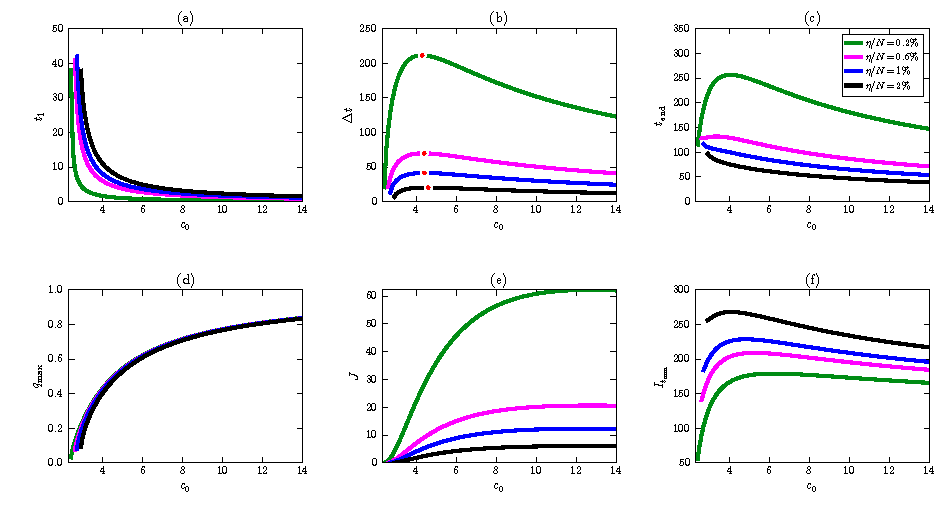
\includegraphics[width=\textwidth]{figures/new4t/S1.pdf}
\caption{基准参数下各指标随常规接触率 $c_0$ 的变化，$\eta/N=0.2\%,0.6\%,1\%,2\%$ 的曲线依次为绿色、品红色、蓝色和黑色，其余参数同正文图~\ref{fig:scenario1:single-sim}；红色圆点为 $\Delta t$ 的数值极大值。(a) 启动时间；(b) 控制时长；(c) 清零时间；(d) 最大隔离比例；(e) 成本 $J$；(f) 总累计新增感染。时间与成本以天计，累计新增感染以人计，$c_0$ 以 $\mathrm d^{-1}$ 计。}
\label{fig:scenario1_summary_c0}
\end{figure}

图~\ref{fig:sup:eta-summary}给出同一组指标随阈值的变化，是正文图~\ref{fig:scenario1_summary_eta}的完整扫描。固定 $c_0$ 时，阈值提高使启动推迟，$q_{\max}$ 只略有下降，控制时长与成本近似与阈值成反比；在所算范围内清零时间缩短，总累计新增感染增加（正文命题~\ref{prop:threshold-tradeoff}）。
\begin{figure}[htbp]
\centering
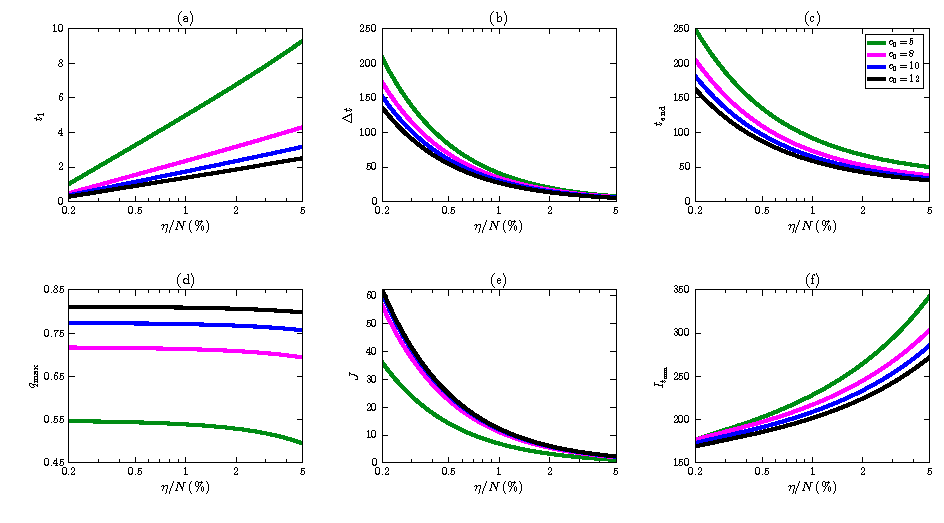
\includegraphics[width=\textwidth]{figures/new4t/S2.pdf}
\caption{基准参数下仅隔离控制的各指标随阈值比例 $\eta/N$ 的变化（横轴为对数刻度），$c_0=5,8,10,12\ \mathrm d^{-1}$ 的曲线依次为绿色、品红色、蓝色和黑色，其余参数同正文图~\ref{fig:scenario1:single-sim}。面板与单位同图~\ref{fig:scenario1_summary_c0}。}
\label{fig:sup:eta-summary}
\end{figure}

图~\ref{fig:baseline:q-joint}给出 $\eta/N=5\%$ 时不同 $c_0$ 与 $c_0=10$ 时不同阈值下的隔离比例轨迹，图~\ref{fig:scenario1_heatmaps_c0_eta}给出 $(\eta/N,c_0)$ 平面上的四项指标。两幅子图中的拐点都在 $\qinf=1-1/[2(1-\beta)]\approx0.4083$ 的同一水平上（正文定理~\ref{thm:s1:inflection}）。$c_0=4$ 时 $q_{\max}=0.3413<\qinf$，即 $S^*<2\bar S$，隔离比例在整个控制期内低于拐点水平，没有内部拐点。

\begin{figure}[htbp]
\centering
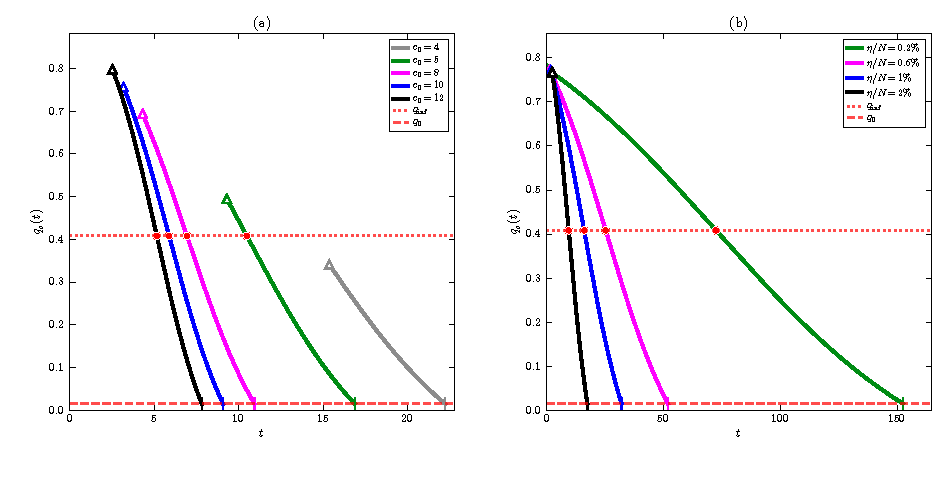
\includegraphics[width=\textwidth]{figures/new4t/S3.pdf}
\caption{不同常规接触率与阈值下仅隔离控制的隔离比例轨迹，其余参数取基准值。(a) $\eta/N=5\%$，$c_0=4,5,8,10,12$ 的曲线依次为灰色、绿色、品红色、蓝色和黑色；(b) $c_0=10$，$\eta/N=0.2\%,0.6\%,1\%,2\%$ 的曲线依次为绿色、品红色、蓝色和黑色。三角形与短竖线分别标出 $t_1$、$t_2$，红点为内部拐点；红色水平虚线为 $q_0$，红色水平点线为 $\qinf\approx0.4083$。}
\label{fig:baseline:q-joint}
\end{figure}

\begin{figure}[htbp]
\centering
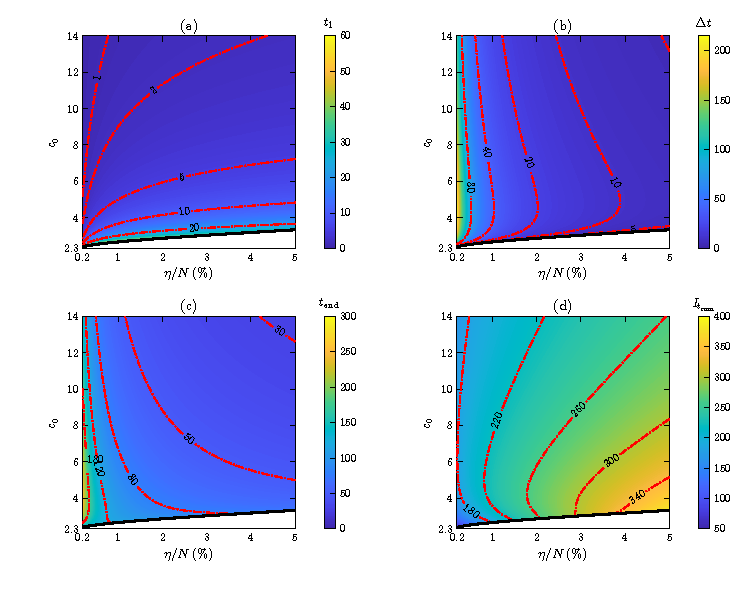
\includegraphics[width=0.8\textwidth]{figures/new4t/S4.pdf}
\caption{$(\eta/N,c_0)$ 平面上仅隔离控制的启动时间、控制时长、清零时间和累计新增感染，其余参数取基准值。黑色实线为触发边界 $c_{0,\min}(\eta)$，白色区域无需加强隔离；红色点划线为等值线，黑色数字为等值。}
\label{fig:scenario1_heatmaps_c0_eta}
\end{figure}

\FloatBarrier
\subsubsection{低阈值极限}
阈值很低时，控制时长与成本按 $1/\theta$ 增长，但这一极限要求初值同时趋于零。固定 $i_0>0$ 时允许的阈值为 $\theta>i_0$，不能在这一问题中直接令 $\theta\to0$。沿同时满足 $i_0\to0$、$\theta\to0$、$0<i_0<\theta$ 的序列，且 $s_0$ 趋于某个大于 $s_c$ 的固定值时，有 $s^*\to s_0$，从而
\begin{equation}
\Delta t\sim\frac1{c_0\theta}\ln\frac{s_0-\bar s}{s_c-\bar s},\qquad
J\sim\frac2{c_0\theta}\int_{s_c}^{s_0}\frac{(1-s_c/s)^2}{s-\bar s}\,ds.
\label{eq:small-threshold}
\end{equation}

相反，固定 $i_0>0$ 而令 $\theta\downarrow i_0$ 时，控制几乎立即启动，控制时长趋于有限值
\[
\frac1{c_0i_0}\ln\frac{s_0-\bar s}{s_c-\bar s}.
\]
因此，由控制时长或成本反解阈值只能在相应的值域内进行，联合小初值极限不能用于固定正初值的问题。

\FloatBarrier

\section{拐点的相对位置}
\label{sec:sup:inflection}

\subsection{参数敏感性}
\label{sec:s1:inflection-position}
内部拐点的相对位置为 $\lambda=(t_{\rm inf}-t_1)/(t_2-t_1)$，定义及存在条件见正文定理\ref{thm:s1:inflection}和式\eqref{eq:s1:lambda}。下列偏导固定其余参数，启动状态 $S^*$ 随所考察的参数变化。
\begin{proposition}
\label{prop:s1:lambda-sensitivity}
在触发条件及 $S_c<2\bar S<S^*$ 下，固定其余参数，有
\[
\frac{\partial\lambda}{\partial\eta}<0,\qquad
\frac{\partial\lambda}{\partial c_0}>0,\qquad
\frac{\partial\lambda}{\partial\beta}>0.
\]
$\partial\lambda/\partial q_0$ 在允许参数域中可正可负，其驻点满足
\begin{equation}
\frac{\ln[(S^*-\bar S)/\bar S]}{(1-q_0)[\beta+q_0(1-\beta)]}
=-\frac{\ln[\bar S/(S_c-\bar S)]}{S^*-\bar S}
\frac{\partial S^*}{\partial q_0}.
\label{eq:s1:lambda-q0-stationary}
\end{equation}
\end{proposition}
\begin{proof}
记 $A=\ln[(S^*-\bar S)/\bar S]>0$、$B=\ln[\bar S/(S_c-\bar S)]>0$，则
\[
\frac{\partial\lambda}{\partial p}
=\frac{B\,\partial A/\partial p-A\,\partial B/\partial p}{(A+B)^2}.
\]
关于 $\eta$，$\partial A/\partial\eta=(\partial S^*/\partial\eta)/(S^*-\bar S)<0$，且 $\partial B/\partial\eta=0$。
关于 $c_0$，
\[
\frac{\partial A}{\partial c_0}=
\frac{\partial S^*/\partial c_0+S^*/c_0}{S^*-\bar S}>0,
\qquad \frac{\partial B}{\partial c_0}=0.
\]
关于 $\beta$，
\[
\frac{\partial A}{\partial\beta}
=\frac{\partial S^*/\partial\beta+S^*/[\beta(1-\beta)]}{S^*-\bar S}>0,
\qquad
\frac{\partial B}{\partial\beta}
=-\frac1{(1-\beta)[\beta+q_0(1-\beta)]}<0.
\]
这些符号给出前三个结论。最后，
\begin{equation}
\frac{\partial\lambda}{\partial q_0}
=\frac1{(A+B)^2}\left[
\frac{B}{S^*-\bar S}\frac{\partial S^*}{\partial q_0}
+\frac{A}{(1-q_0)[\beta+q_0(1-\beta)]}\right].
\label{eq:lambda-q0-sign}
\end{equation}
令方括号为零得到驻点条件。两项异号本身不足以说明导数能取两种符号；第\ref{app:lambda}节给出两个满足全部条件的参数点，并分别证明其导数为正和负。
\end{proof}

拐点总出现在 $S=2\bar S$ 处，$A$、$B$ 分别与 $S$ 从 $S^*$ 降到 $2\bar S$、从 $2\bar S$ 降到 $S_c$ 所需的时间成正比，$\lambda=A/(A+B)$。提高 $\eta$ 使 $S^*$ 减小、前一段缩短，拐点因而在控制期中提前。符号结果汇总于正文附录表~\ref{tab:sensitivity}。

\subsection{数值结果}
图~\ref{fig:s1:lambda-sensitivity}中，$\lambda$ 随 $\eta$ 增大而减小，随 $c_0$ 和 $\beta$ 增大而增大，与命题~\ref{prop:s1:lambda-sensitivity}一致。$\lambda$ 对 $q_0$ 的依赖不单调：取 $c_0=10$、$\eta/N=0.05$，其余参数取基准值，在 $q_0\in[0,0.39]$ 内 $\lambda$ 有局部极大值，其位置 $q_0^\dagger$ 随 $\beta$ 增大而增大，
\[
\begin{array}{c|ccc}
\beta & 0.10 & 0.12 & 0.155\\
\hline
q_0^\dagger
&0.0736525&0.1969606&0.3890712
\end{array}
\]
三个位置两侧的 $\partial\lambda/\partial q_0$ 均由正变负。

\begin{figure}[htbp]
\centering
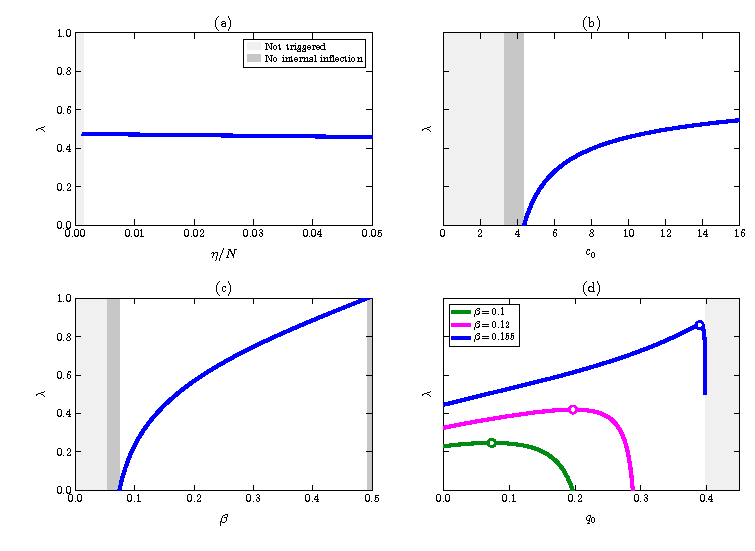
\includegraphics[width=0.8\textwidth]{figures/new4t/S5.pdf}
\caption{拐点相对位置 $\lambda$ 随 $\eta/N$、$c_0$、$\beta$、$q_0$ 的变化，其余参数取基准值，基准曲线为蓝色；$q_0$ 面板比较 $\beta=0.10,0.12,0.155$，曲线依次为绿色、品红色和蓝色，其灰色区域对应 $\beta=0.155$。空心圆为局部极大值；浅灰区域不满足触发条件，深灰区域已触发控制但没有内部拐点。}
\label{fig:s1:lambda-sensitivity}
\end{figure}

图中的灰色区域是内部拐点存在条件 $S_c<2\bar S<S^*$ 的边界：改变 $\beta$ 时两侧的边界都可能出现，改变 $c_0$ 时内部拐点在 $S^*=2\bar S$ 处出现；在图示的 $q_0$ 与 $\eta/N$ 范围内，只要控制被触发，内部拐点就存在。不同 $c_0$ 与阈值下的隔离比例轨迹见图~\ref{fig:baseline:q-joint}。另一侧的边界由 $\qinf=q_0$ 给出：西安参数的 $q_0=0.3230$ 下由此得 $\beta_{\max}=0.261448$，$\beta$ 超过该值时 $\qinf<q_0$，内部拐点不再存在。

\FloatBarrier
\subsection{变号的构造}
\label{app:lambda}
为说明式\eqref{eq:lambda-q0-sign}确实可正可负，取
\[
N=10^6,\quad \beta=\frac16,\quad q_0=\frac1{10},\quad
\gamma=\frac1{10},\quad c_0=\frac{20}{3},\quad I_0=100.
\]
此时 $\beta_2^0/\beta_1^0=3/5,S_c=N/10,\bar S=3N/40$。固定 $S^*=N/5$，对 $m\in\{21/20,2\}$ 分别构造
\[
S_0=mS^*,\qquad
\eta=I_0+\frac{\beta_2^0}{\beta_1^0}(S_0-S^*)+\rho_1\ln(S^*/S_0).
\]
两组参数均有 $S_0+I_0<N$、$I_0<\eta<I_{\max}^{0}$ 和 $S_c<2\bar S<S^*$，余下的初始人数置于不参与社区传播的仓室（如 $R(0)>0$）；正文第~\ref{sec:model}~节只要求初始仓室非负、总和为 $N$，因而允许这种初值。在每个构造出的参数点求偏导时，固定该点的 $S_0,\eta$；以上关系只用于构造参数点，不作为求导时的约束。

代入式\eqref{eq:lambda-q0-sign}，得到
\begin{equation}
\frac{\partial\lambda}{\partial q_0}
=\frac{40}{9(\ln5)^2}
\left[\ln\frac53-\ln3\left(\frac{16}{5}(m-1)-\frac65\ln m\right)\right].
\end{equation}
当 $m=21/20$ 时，圆括号中的量在 $0$ 与 $4/25$ 之间。结合 $\ln(5/3)>2/5$、$\ln3<2$，方括号大于 $2/25>0$。当 $m=2$ 时，圆括号中的量大于 $2$；由 $\ln3>2/3$、$\ln(5/3)<2/3$，方括号严格为负。这些估计均可由 $(x-1)/x<\ln x<x-1$（$x>1$）得到，故两种符号都在允许参数域中出现。

\section{显式控制族}
\label{sec:sup:explicit}
正文式\eqref{eq:joint:explicit-c}--\eqref{eq:joint:explicit-q}定义了一族连接两种单控制的控制。本节给出这一族的状态轨迹、控制时长及能力约束下的允许范围。
\begin{theorem}
\label{thm:joint:explicit}
固定 $0<\alpha\le1$ 时，式\eqref{eq:joint:explicit-c}--\eqref{eq:joint:explicit-q}对应的阈值控制期状态为
\begin{equation}
S(t)=S_c+
\left(S^*-S_c+\frac{S_c-\bar S}{\alpha}\right)
 e^{-\frac{c_0\eta\alpha}{N}(t-t_1)}
-\frac{S_c-\bar S}{\alpha},\qquad I(t)=\eta,
\label{eq:joint:explicit-S}
\end{equation}
控制时长为
\begin{equation}
\Delta t(\alpha)=\frac{N}{c_0\eta\alpha}
\ln\!\left(1+\frac{\alpha(S^*-S_c)}{S_c-\bar S}\right).
\label{eq:joint:explicit-duration}
\end{equation}
$\alpha=0$ 时，相应表达为
\begin{equation}
S(t)=S^*-\frac{c_0\eta}{N}(S_c-\bar S)(t-t_1),\qquad
\Delta t(0)=\frac{N(S^*-S_c)}{c_0\eta(S_c-\bar S)}.
\label{eq:joint:explicit-zero}
\end{equation}
将上述 $S(t)$ 代入式\eqref{eq:joint:explicit-c}--\eqref{eq:joint:explicit-q}，即得到两个控制的时间表达。$\alpha=0$ 对应仅减少接触，$\alpha=1$ 恢复第~\ref{sec:s1}~节的仅隔离控制。对于 $0<\alpha<1$，阈值控制期内接触率严格增加、隔离比例严格下降，并在退出时同时连续恢复为 $(c_0,q_0)$。
\end{theorem}
\begin{proof}
代入式\eqref{eq:joint:Sdot}得
\[
\dot S=-\frac{c_0\eta}{N}\bigl[S_c-\bar S+\alpha(S-S_c)\bigr],
\qquad S(t_1)=S^*.
\]
分别求解 $\alpha>0$ 和 $\alpha=0$ 的线性方程，得到状态表达；令 $S(t_2)=S_c$ 得到控制时长。两组公式在 $\alpha\downarrow0$ 时连续衔接。对于 $0<\alpha<1$，
\[
\frac{\partial c_c(S;\alpha)}{\partial S}
=-\frac{c_0(1-\alpha)S_c}{S^2}<0,\qquad
\frac{\partial q_c(S;\alpha)}{\partial S}
=\frac{(1-q_0)S_c\alpha}{[S_c+\alpha(S-S_c)]^2}>0,
\]
结合 $\dot S<0$ 即得时间单调性。代入 $S=S_c$ 得到退出值，代入 $\alpha=0,1$ 分别恢复两种单控制。
\end{proof}
\begin{corollaryn}
\label{cor:joint:allocation-range}
在能力约束下，上述显式族可行当且仅当
\begin{equation}
\max\!\left\{0,\frac{c_{\min}S^*-c_0S_c}{c_0(S^*-S_c)}\right\}
\le\alpha\le
\min\!\left\{1,\frac{S_c(q_{\rm cap}-q_0)}{(1-q_{\rm cap})(S^*-S_c)}\right\}.
\label{eq:joint:allocation-range}
\end{equation}
该区间非空当且仅当式\eqref{eq:joint:feasibility}成立。
\end{corollaryn}
\begin{proof}
显式族中 $c$ 不减、$q$ 不增，故只需在 $S=S^*$ 处检查 $c\ge c_{\min}$ 和 $q\le q_{\rm cap}$。代入式\eqref{eq:joint:explicit-c}--\eqref{eq:joint:explicit-q}并与 $\alpha\in[0,1]$ 取交，得到式\eqref{eq:joint:allocation-range}。未截断的下界不超过 $1$，未截断的上界非负；二者的大小关系等价于
$c_{\min}S^*\le c_0(1-q_0)S_c/(1-q_{\rm cap})$，
即式\eqref{eq:joint:feasibility}，故该区间与 $\mathcal A(\eta;c_{\min},q_{\rm cap})$ 同时非空。
\end{proof}

\section{权重结构的补充分析}
\label{sec:sup:weight-structure}

\subsection{网格与分类}
正文图~\ref{fig:joint:phase}在 $r\in[0.9,20]$ 的 $300$ 个对数等距点与 $S\in(S_c,S^*]$ 的 $300$ 个等距点上逐状态求解，正文讨论其中 $r\ge1$ 的部分，跳变位置在 $S$ 上二分定位；默认的 $r=2$ 由正文第~\ref{sec:joint:compare-numerics}~节单独计算。表~\ref{tab:joint:weight-transitions}给出成本最优控制的结构转折所在的 $r$ 括区。括区由 $r\in[0.1,20]$ 内 $161$ 个对数等距点的原网格出发确定：对全部网格点重新分类，在类别不同的相邻网格点之间取 $20$ 个细分点，找出每个改变区间，再在 $\log r$ 上二分到宽度小于 $10^{-3}$，不假定结构类别对 $r$ 单调；各括区在 $N_z=8001$ 与 $16001$ 下类别不变。结构 A$'$ 中的内部跳变另用不依赖根法的 $2\times10^{5}$ 点网格逐点核对：两个内部局部极小在跳变处交换全局最优，两个分支的成本相对只差约 $10^{-5}$。

\subsection{结构边界}
表~\ref{tab:joint:weight-transitions}的前两个转折可以与闭式比较。正文定理~\ref{thm:joint:cost-structure}的权重界 $r_{\rm cont}$（式\eqref{eq:joint:rcont}）保证控制连续，两组参数下的值都落在 A$\to$A$'$ 的括区内；A$'\to$B 的转折由下面的命题给出。
\begin{proposition}
\label{prop:sup:rhat}
设 $w_c,w_q>0$，$r=w_q/w_c$，不考虑能力约束。对一切 $S>S_{\rm sw}$，$c=c_0$ 都是 $f(S,\cdot)$ 在 $[c_0S_c/S,c_0]$ 上的唯一全局最小点，当且仅当
\[
r\le\hat r=\Bigl(\frac{S_{\rm sw}}{S_{\rm sw}-S_c}\Bigr)^2 .
\]
此外 $9/4<\hat r<4$，且 $r_{\rm cont}<\hat r$。
\end{proposition}
\begin{proof}
沿用正文附录~\ref{sec:proof:cost-structure}的记号 $\zeta,p,G=A+rB$。先证上集性：若 $p=\zeta_0$ 是 $G(\cdot;\zeta_0)$ 的全局最小点，则对任意 $\zeta_1>\zeta_0$，$p=\zeta_1$ 是 $G(\cdot;\zeta_1)$ 的唯一全局最小点。由正文命题~\ref{prop:joint:global-structure}，$\zeta_0\ge\zeta_{\rm sw}$。对固定 $p<\zeta$，$A$ 关于 $\zeta$ 严格增；$B$ 与 $\zeta$ 无关，且 $B'(p)=-(p-1)(p^2-3p+2b)/[p^3(p-b)^2]$，故 $B$ 在 $[\zeta_{\rm sw},\infty)$ 上严格减。$p\le\zeta_0$ 时，$G(p;\zeta_1)>G(p;\zeta_0)\ge rB(\zeta_0)\ge rB(\zeta_1)=G(\zeta_1;\zeta_1)$；$\zeta_0<p<\zeta_1$ 时，$G(p;\zeta_1)\ge rB(p)>rB(\zeta_1)$。

再看 $S_{\rm sw}$ 处。令 $x=c/c_0\in[\sigma,1]$，$\sigma=S_c/S$，$a=(1-\sigma)^2$，$d=1-b\sigma$。利用恒等式 $d(x-\sigma)^2-ax^2(x-b\sigma)=(1-x)P(x)$，$P(x)=ax^2-d\sigma(2-\sigma)x+d\sigma^2$，对 $x\in[\sigma,1)$，$f(S,c_0x)\ge f(S,c_0)$ 等价于 $d(1-x)x^2+rP(x)\ge0$。在 $\sigma=S_c/S_{\rm sw}$ 上 $2b\sigma^2-3\sigma+1=0$，即 $2\sigma d=1-\sigma$，于是 $P(x)=a(x-1)(x-x_2)$，$x_2=\sigma/[2(1-\sigma)]<\sigma$。条件化为：对一切 $x\in[\sigma,1)$ 有 $r(x-x_2)\le(d/a)x^2$。比值 $(d/a)x^2/(x-x_2)$ 在 $x=2x_2=\sigma/(1-\sigma)\in(\sigma,1)$ 取最小值 $4x_2d/a=1/(1-\sigma)^2=\hat r$。

若 $r<\hat r$，$c_0$ 是 $S_{\rm sw}$ 处的唯一全局最小点；若 $r=\hat r$，它与 $x=2x_2$ 并列。两种情形下，由上集性，对一切 $S>S_{\rm sw}$，$c_0$ 都是唯一全局最小点。若 $r>\hat r$，则在 $S_{\rm sw}$ 处存在 $x<1$ 使 $f(S,c_0x)<f(S,c_0)$；由连续性，这一严格不等式在 $S_{\rm sw}$ 稍上方仍成立。最后，$S_{\rm sw}/S_c\in(2,3)$ 给出 $9/4<\hat r<4$；由 $\zeta_{\rm sw}=S_{\rm sw}/S_c$ 得 $b=\zeta_{\rm sw}(3-\zeta_{\rm sw})/2$，不等式 $r_{\rm cont}<\hat r$ 化为 $(\zeta_{\rm sw}-1)(\zeta_{\rm sw}-2)^2>0$。
\end{proof}
$\hat r$ 的含义是：隔离的相对权重超过它以后，在 $S_{\rm sw}$ 稍上方同时减少接触已经更省；若存在仅隔离段，它就会在到达 $S_{\rm sw}$ 前结束。
\begin{table}[htbp]
\centering\small
\renewcommand{\arraystretch}{1.2}
\begin{threeparttable}
\caption{权重网格上成本最优控制的结构转折}
\label{tab:joint:weight-transitions}
\begin{tabular*}{\linewidth}{@{\extracolsep{\fill}}llcccc@{}}
\toprule
 & & \multicolumn{2}{c}{基准} & \multicolumn{2}{c}{西安}\\
\cmidrule(lr){3-4}\cmidrule(l){5-6}
转折 & 结构变化 & 闭式 & 括区 & 闭式 & 括区\\
\midrule
A$\to$A$'$ & 出现内部跳变 & $r_{\rm cont}=\nrCostRcontBase$ & $[\nrWtBaseAToApLo,\nrWtBaseAToApHi]$ & $r_{\rm cont}=\nrCostRcontXian$ & $[\nrWtXianAToApLo,\nrWtXianAToApHi]$\\
A$'\to$B & 切换提前并跳变 & $\hat r=\nrCostRhatBase$ & $[\nrWtBaseApToBLo,\nrWtBaseApToBHi]$ & $\hat r=\nrCostRhatXian$ & $[\nrWtXianApToBLo,\nrWtXianApToBHi]$\\
B$\to$C & 仅隔离段消失 & — & $[\nrWtBaseBToCLo,\nrWtBaseBToCHi]$ & — & $[\nrWtXianBToCLo,\nrWtXianBToCHi]$\\
\bottomrule
\end{tabular*}
\begin{tablenotes}[flushleft]\footnotesize
\item 注：$w_c=1$，$r=w_q/w_c$，不考虑能力约束。结构 A：在 $S_{\rm sw}$ 处连续切换，此后控制连续；A$'$：在 $S_{\rm sw}$ 处连续切换，随后在 $S_{\rm sw}$ 稍下方于两个内部取值之间跳变一次；B：切换提前到 $S_{\rm sw}$ 以上，接触率在切换处跳变；C：没有仅隔离段。括区是所检验网格与精度下含该转折的 $r$ 括区，宽度小于 $10^{-3}$；闭式列中 $r_{\rm cont}$ 为正文定理~\ref{thm:joint:cost-structure}的连续界（充分条件），$\hat r$ 见命题~\ref{prop:sup:rhat}。
\end{tablenotes}
\end{threeparttable}
\end{table}

图~\ref{fig:sup:phase-detail}放大正文图~\ref{fig:joint:phase}的转折区。数值上，内部跳变从 $r=r_{\rm cont}$ 处开始（空心圆），连续切换与由仅隔离控制出发的跳变在 $(S_{\rm sw},\hat r)$ 处相接（空心菱形）。
\begin{figure}[htbp]
\centering
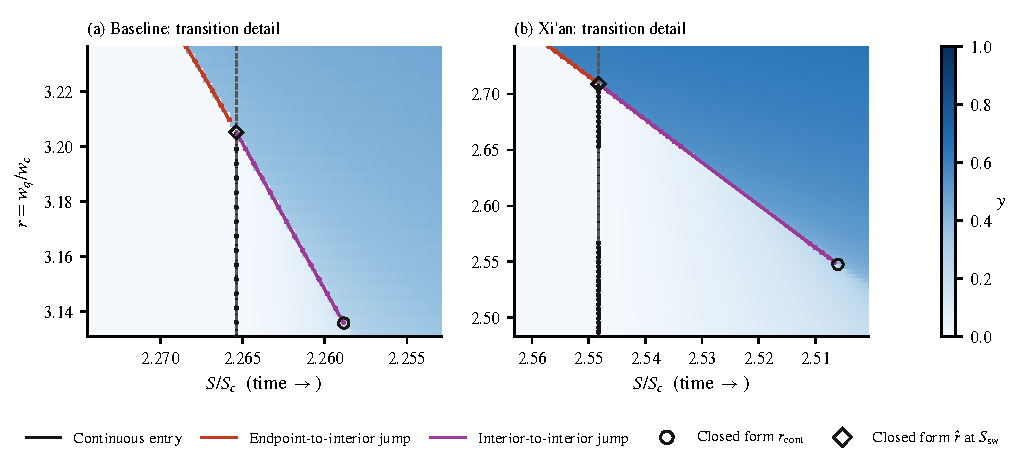
\includegraphics[width=\textwidth]{figures/joint_v2/joint_phase_detail.pdf}
\caption{正文图~\ref{fig:joint:phase}转折区的局部加密。(a) 基准参数；(b) 西安参数。颜色为 $y$；点为表~\ref{tab:joint:weight-transitions}所涉加密权重及西安两处补充计算点上的局部分类，黑线为连续进入内部分支的边界，红线为端点到内部的跳变，紫线为两个内部取值之间的跳变。空心圆位于 $r=r_{\rm cont}$（正文式\eqref{eq:joint:rcont}）、$S/S_c=b+\sqrt{b^2-8b+8}$，空心菱形为 $(S_{\rm sw}/S_c,\hat r)$（命题~\ref{prop:sup:rhat}）。随时间推进，$S$ 从左向右减小。}
\label{fig:sup:phase-detail}
\end{figure}
\FloatBarrier

\Needspace{12\baselineskip}
\section{西安算例的补充结果}
\label{sec:sup:xian}
西安参数见正文表~\ref{tab:xian_initial_fit}，计算使用 $I_0$ 的未取整值。

\subsection{人口缩放}
\label{sec:sup:xian:settings}
人口缩放情景取 $N=N_{\rm eff}$、$S_0=N-I_0$，沿用全市拟合的绝对初值 $I_0$ 与传播参数，其余初始仓室为零，不重新拟合。它同时改变 $N$、$i_0=I_0/N$ 与 $\eta=\theta N$。固定 $\theta=0.002$、取 $N\in\{5\times10^4,10^5,5\times10^5,10^6,5\times10^6,1.3163\times10^7\}$ 的六个人口规模，仅隔离控制的控制时长均约为 $85.07$ 天，$\Delta t$ 和 $J$ 的相对极差分别为 $4.71\times10^{-8}$ 和 $1.17\times10^{-7}$；以 $t-t_1$ 为时间变量时，归一化感染轨迹和隔离比例近似重合。启动时间由 $11.39$ 天增加至 $16.90$ 天，这是固定绝对初值时，初始感染比例 $i_0=I_0/N$ 随 $N$ 增大而减小的结果：初期近似指数增长，$t_1\approx g^{-1}\ln(\theta/i_0)$，其中 $g=\beta c_0(1-q_0)-\gamma$ 为初期增长率。固定绝对阈值 $\eta=100$、把 $N$ 从 $1.3163\times10^7$ 降到 $5\times10^4$ 时，$\theta=\eta/N$ 增大，控制时长由约 $2.25\times10^4$ 天缩短到约 $85$ 天。两组结果都符合
\[
\Delta t=\frac1{c_0\theta}\ln\frac{s^*-\bar s}{s_c-\bar s},
\]
其中对数因子在 $\theta\in[5\times10^{-4},8\times10^{-3}]$ 内仅由 $2.20$ 变到 $2.15$，因此 $\Delta t$ 近似与 $\theta$ 成反比。

固定归一化初值时，以绝对终点 $I=1$ 计的量随人口单调变化。记 $i_{\max}^{0}=I_{\max}^{0}/N$（式\eqref{eq:s1:Imax-no}），固定归一化初值 $s_0,i_0$ 时它不依赖 $N$。
\begin{proposition}
\label{prop:reference-population}
固定 $s_0,i_0,\theta$ 和模型参数，且 $i_0<\theta<i_{\max}^{0}$。在 $N\theta>1$ 的范围内，仅隔离控制的清零时间、计算至该终点的累计新增感染及其占人口的比例均随 $N$ 严格增加。
\end{proposition}
\begin{proof}
归一化轨迹及启动、控制时长与 $N$ 无关。退出后 $i(t)$ 从 $\theta$ 严格下降至零，终点为 $i=1/N$。增大 $N$ 使终点更低，故清零时间严格增加。

记 $s_{\rm end}=S_{\rm end}/N$。归一化的退出后首次积分为
\[
\frac1N=\theta+\frac{\beta_2^0}{\beta_1^0}(s_c-s_{\rm end})
+\frac{\rho_1}{N}\ln\frac{s_{\rm end}}{s_c},
\]
其中 $\rho_1/N$ 与 $\beta_2^0/\beta_1^0$ 均不随 $N$ 改变。于是
\[
\frac{\partial s_{\rm end}}{\partial N}
=-\frac1{N^2(\rho_1/N)(1/s_{\rm end}-1/s_c)}<0.
\]
将式\eqref{eq:s1:cumulative}除以 $N$ 后，只有 $s_{\rm end}$ 含 $N$，因而比例满足
\[
\frac{\partial(\Itcum/N)}{\partial N}
=-\frac{\beta}{\beta+q_0(1-\beta)}\frac{\partial s_{\rm end}}{\partial N}>0,
\]
人数满足
\[
\frac{\partial\Itcum}{\partial N}
=\frac{\Itcum}{N}
-\frac{N\beta}{\beta+q_0(1-\beta)}\frac{\partial s_{\rm end}}{\partial N}>0.\qedhere
\]
\end{proof}
命题不适用于固定绝对阈值或固定绝对 $I_0$ 的比较，后者见上一段。

\FloatBarrier
\subsection{阈值扫描}
\label{sec:sup:xian:threshold-scan}
表~\ref{tab:sup:eta}与图~\ref{fig:xian_eta_sens}给出 11 个阈值比例下仅隔离控制的结果，覆盖设计阈值 $\eta/N=0.002$ 的两侧。阈值从 $0.01N$ 降到 $0.0001N$ 时，$q_{\max}$ 只在 $0.838$ 与 $0.847$ 之间变化，控制时长与成本近似按阈值的反比增加，总累计新增感染则缓慢减少；正文第~\ref{sec:xian:threshold-scale}~节由此解释低阈值的代价。
\begin{table}[htbp]
\centering\small
\setlength{\tabcolsep}{3.5pt}
\renewcommand{\arraystretch}{1.25}
\begin{threeparttable}
\caption{西安参数下不同阈值的仅隔离控制}
\label{tab:sup:eta}
\begin{tabular*}{\linewidth}{@{\extracolsep{\fill}}S[table-format=1.4]S[table-format=1.4]S[table-format=4.2]S[table-format=4.2]S[table-format=3.4]S[table-format=7.0]@{}}
\toprule
{$\eta/N$} & {$q_{\max}$} & {$\Delta t$（d）} & {$t_{\rm end}$（d）} & {$J$（d）} & {\shortstack{总累计新增感染\\（人）}}\\
\midrule
0.0001 & 0.8470 & 1710.66 & 2209.55 & 826.4066 & 2155649\\
0.0002 & 0.8469 & 855.09 & 1243.15 & 412.9141 & 2182123\\
0.0005 & 0.8466 & 341.75 & 620.77 & 164.8184 & 2234666\\
0.0010 & 0.8462 & 170.63 & 389.32 & 82.1192 & 2293939\\
0.0015 & 0.8458 & 113.59 & 304.01 & 54.5524 & 2339486\\
0.0020 & 0.8454 & 85.07 & 258.10 & 40.7686 & 2377943\\
0.0030 & 0.8445 & 56.55 & 208.39 & 26.9842 & 2442608\\
0.0040 & 0.8436 & 42.29 & 181.18 & 20.0913 & 2497306\\
0.0050 & 0.8428 & 33.73 & 163.65 & 15.9550 & 2545663\\
0.0075 & 0.8405 & 22.32 & 138.10 & 10.4383 & 2649240\\
0.0100 & 0.8382 & 16.61 & 123.89 & 7.6781 & 2737382\\
\bottomrule
\end{tabular*}
\begin{tablenotes}[flushleft]\footnotesize
\item 注：$q_{\max}=q_c(t_1)$；$\eta/N$ 为比例，$0.002$ 即 $0.2\%$；总累计新增感染计算至清零时间。
\end{tablenotes}
\end{threeparttable}
\end{table}

\begin{figure}[htbp]
    \centering
    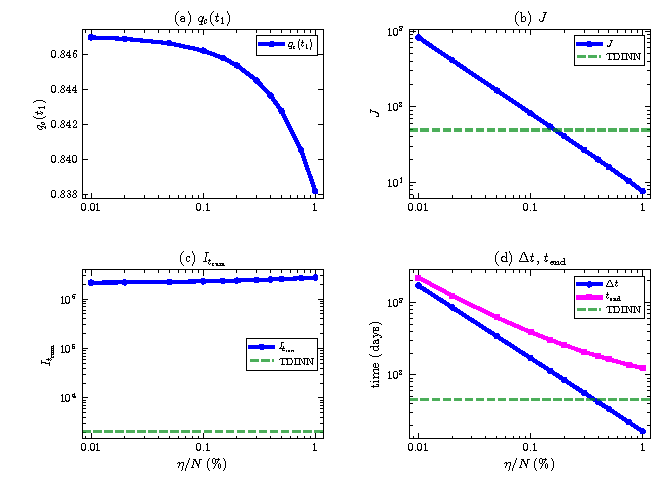
\includegraphics[width=0.7\textwidth]{new4o/xian_eta_sensitivity.pdf}
    \caption{西安参数下仅隔离控制的指标随 $\eta/N$ 的变化：(a) 启动时的隔离比例；(b) 成本 $J$；(c) 累计新增感染；(d) 控制时长与清零时间。水平虚线为 TDINN 参照值，其中 TDINN 的 $J$ 用同一二次强度被积函数与默认权重在 $[0,t_{\rm end}^{\rm T}]$ 上积分；(d) 中 TDINN 的控制时长与清零时间同为 $45.29$ d。}
    \label{fig:xian_eta_sens}
\end{figure}

图~\ref{fig:xian_heatmaps}把扫描推广到 $(\eta,c_0)$ 平面。在图示的 $c_0$ 范围内，控制时长、清零时间与成本的等值线接近竖直，主要由阈值决定；正文第~\ref{sec:xian:threshold-scale}~节在 TDINN 峰值处的控制时长即取自子图 (a)。
\begin{figure}[htbp]
    \centering
    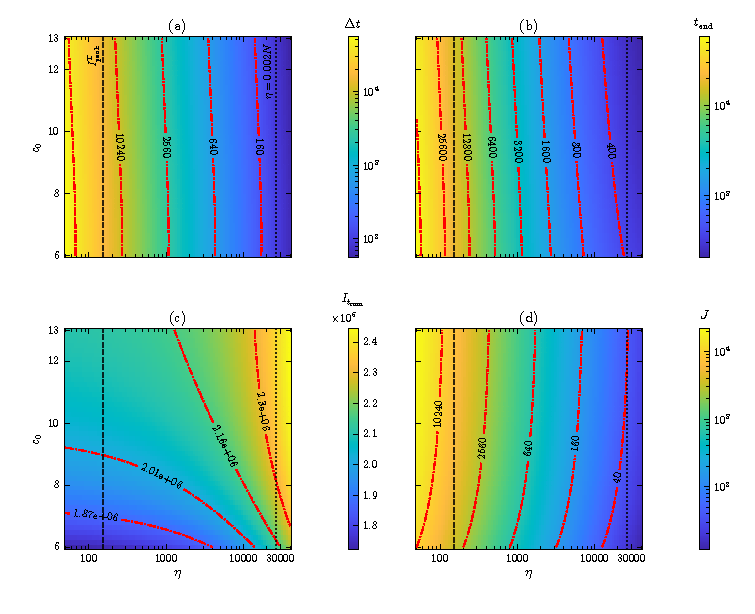
\includegraphics[width=0.8\textwidth]{figures/new4t/S8.pdf}
    \caption{西安参数下仅隔离控制在 $(\eta,c_0)$ 平面上的指标：(a) 控制时长；(b) 清零时间；(c) 累计新增感染；(d) 成本 $J$。两条竖直参照线分别为 TDINN 的非隔离感染者峰值 $\eta=152.55$ 与设计阈值 $\eta=26326$；红色点划线为等值线，黑色数字为等值。}
    \label{fig:xian_heatmaps}
\end{figure}

\subsection{设计阈值的量级}
\label{sec:sup:threshold-scale}
正文西安算例取 $N=13{,}163{,}000$\cite{XianStat2021}、$\eta=0.002N=26{,}326$。这一阈值来自下面的量级估计，它与第~\ref{sec:sup:medical-link}~节的充分条件是两种不同的依据。

陈胤孜等\cite{Chen2021ICUForecast}基于既往资料预测，2021 年全国每10万人综合 ICU 床位约为 $4.37$ 张；这一数值为全国预测量，而非西安同期可用容量的实测值。Angulo 等\cite[补充材料 S4.1]{Angulo2021}对早期 COVID-19 采用需要重症监护的感染者比例名义值 $0.60\times0.15\times0.28=0.0252$。将前者作为人均容量参考、不扣除既有占用，并将后者移作参考系数 $\rho_{\mathrm{ICU}}$，按比例情景
\[
\eta=\frac{C}{\rho_{\mathrm{ICU}}},\qquad
\theta=\frac{C/N}{\rho_{\mathrm{ICU}}}
\]
得到
\[
\theta=\frac{4.37/10^5}{0.0252}\approx1.73\times10^{-3},
\qquad \eta\approx2.28\times10^4.
\]
正文在这一量级附近取 $\theta=0.002$ 作为设计情景。按相同的参考系数反算，它对应每10万人 $5.04$ 张、全市约 $663$ 张的名义容量。

这一比例移植只给出阈值的量级，不是当地医疗容量的临床校准。以确诊病例或全部感染者为分母的 ICU 入院风险可能不同\cite{Pung2023Undetected}；参考系数 $\rho_{\mathrm{ICU}}$ 也没有依据共同的需求函数和初始负担估计，不等同于第~\ref{sec:sup:medical-link}~节中的 $pL\beta c_0S_0/N$。

\FloatBarrier

\section{隔离易感者回流}
\label{sec:sup:return}
正文研究隔离易感者在清零前不释放的情形（第~\ref{sec:model}~节）。本节用数值说明：若被隔离的未感染者在疫情过程中陆续返回社区，正文的哪些结论仍成立，哪些会改变。

\subsection{模型与设定}
含回流的模型在式\eqref{eq:model:full}的 $S$、$S_q$ 方程中加入回流项 $\omega S_q$：
\begin{equation}
\begin{cases}
\dot S=-\dfrac{c[\beta+(1-\beta)q]}{N}SI+\omega S_q,\\[.5em]
\dot I=\dfrac{\beta c(1-q)}{N}SI-\gamma I,\\[.5em]
\dot S_q=\dfrac{(1-\beta)cq}{N}SI-\omega S_q,\\[.5em]
\dot I_q=\dfrac{\beta cq}{N}SI-\delta_q I_q,\\[.5em]
\dot R=\gamma I+\delta_q I_q,
\end{cases}
\qquad\omega\ge0.
\label{eq:return:model}
\end{equation}
回流率 $\omega$ 为常数，隔离易感者的停留时间服从均值 $1/\omega$ 的指数分布，$\omega=0$ 即式\eqref{eq:model:full}。本节取 $1/\omega=14$ d，与既有隔离时长研究涉及的时间尺度相近\cite{Ashcroft2021,Wells2021}。指数停留是简化的回流机制，与固定期限或检测后解除不同。

阈值策略的实施方式与正文相同。$I$ 首次到达 $\eta$ 时启动；此后取 $c_0S_c/S\le c\le c_0$，隔离比例由平衡式\eqref{eq:model:balance}确定，从而维持 $I\equiv\eta$；$S$ 首次降到 $S_c$ 时恢复 $(c_0,q_0)$ 并一直保持。退出时不额外释放隔离易感者，$S_q$ 继续按回流机制演化，退出后也不重新启动干预。有回流时阈值控制期内的 $S$ 可能回升，上述接触率范围对 $S\ge S_c$ 照样适用。两组参数的初值同正文，$S_q(0)=0$。累计新增感染计至退出后 $I$ 首次降到 $1$ 的时刻
\begin{equation}
T_{\rm cut}=\inf\{t>t_2:I(t)=1,\ \dot I(t)<0\},
\label{eq:return:cut}
\end{equation}
与正文清零时间的约定相同。

追踪与回流只在 $S$ 与 $S_q$ 之间转移人数。两式相加，总易感者 $U=S+S_q$ 满足 $\dot U=-\beta cSI/N$，因此
\begin{equation}
\Itcum(T)=U(0)-U(T).
\label{eq:return:U}
\end{equation}

比较五种控制：仅隔离控制、仅减少接触、无回流成本最优律（正文定理~\ref{thm:joint:cost-minimum}的状态反馈，$w_c=1$、$w_q=2$，直接用于回流模型），以及在回流模型中重新优化的控制时长最短与成本 $J$ 最低的控制。重新优化在阈值策略内进行，用时间域 Radau 配点，区间数由 $20$ 逐级加密到 $160$，粗网格取十个起点。最终候选用完整五仓室方程回放核验，并用分段常控制的打靶法复核。

\subsection{数值结果}
回流下控制时长最短的控制收敛到仅隔离控制，表~\ref{tab:sup:return:term}中不再单列。
\begin{table}[htbp]
\centering\small
\renewcommand{\arraystretch}{1.2}
\begin{threeparttable}
\caption{平均停留 $14$ d 的指数回流情景下各控制的结果}
\label{tab:sup:return:term}
\begin{tabular*}{0.8\linewidth}{@{\extracolsep{\fill}}lccc@{}}
\toprule
控制 & $\Delta t$（d） & $J$（d） & $\Itcum(T_{\rm cut})$\\
\midrule
\multicolumn{4}{@{}l}{基准参数（人）}\\
仅隔离控制 & $\nrRwBaseQDt$ & $\nrRwBaseQJ$ & $\nrRwBaseQInf$\\
回流下的成本最优控制 & $\nrRwBaseODt$ & $\nrRwBaseOJ$ & $\nrRwBaseOInf$\\
无回流成本最优律 & $\nrRwBaseMDt$ & $\nrRwBaseMJ$ & $\nrRwBaseMInf$\\
仅减少接触 & $\nrRwBaseCDt$ & $\nrRwBaseCJ$ & $\nrRwBaseCInf$\\
\midrule
\multicolumn{4}{@{}l}{西安参数（$\eta=0.001N$，$10^6$ 人）}\\
仅隔离控制 & $\nrRwXianQDt$ & $\nrRwXianQJ$ & $\nrRwXianQInf$\\
回流下的成本最优控制 & $\nrRwXianODt$ & $\nrRwXianOJ$ & $\nrRwXianOInf$\\
无回流成本最优律 & $\nrRwXianMDt$ & $\nrRwXianMJ$ & $\nrRwXianMInf$\\
仅减少接触 & $\nrRwXianCDt$ & $\nrRwXianCJ$ & $\nrRwXianCInf$\\
\bottomrule
\end{tabular*}
\begin{tablenotes}[flushleft]\footnotesize
\item 注：$1/\omega=14$ d；$\Itcum(T_{\rm cut})$ 见式\eqref{eq:return:cut}；$J$ 取 $w_c=1$、$w_q=2$。
\end{tablenotes}
\end{threeparttable}
\end{table}

正文的结构性结论在这一情景中仍成立：
\begin{itemize}
\item 仅隔离控制的控制时长最短，仅减少接触最长；
\item 回流下的成本最优控制先仅隔离（基准约前 $\nrRwBaseFrontPct\%$、西安约前 $\nrRwXianFrontPct\%$ 的控制期），随后两种措施并用；直接沿用无回流成本最优律，成本只高约 $\nrRwBaseMigGapPct\%$ 与 $\nrRwXianMigGapPct\%$；
\item 各控制退出后 $I$ 都未越过 $\eta$。
\end{itemize}

改变的是量级。仅隔离控制的控制时长由无回流的 $\nrRwBaseQDtNoret$ d 与 $\nrRwXianQDtNoret$ d 增至 $\nrRwBaseQDt$ d 与 $\nrRwXianQDt$ d。累计新增感染接近 $U(0)-S_c$，后者基准为 $\nrRwBaseL$ 人、西安为 $\nrRwXianL\times10^6$ 人。控制之间的感染差别也明显缩小：仅减少接触比仅隔离控制多出的感染，基准参数下由无回流时的约 $\nrRwBaseDiffPctNoret\%$ 降到约 $\nrRwBaseDiffPct\%$，西安参数下由约 $\nrRwXianDiffPctNoret\%$ 降到约 $\nrRwXianDiffPct\%$。

原因在于终止时总易感者已低于常规传播临界值：各轨迹在 $T_{\rm cut}$ 时 $U/S_c$ 在基准参数下为 $\nrRwBaseUMin$--$\nrRwBaseUMax$，西安参数下约为 $\nrRwXianUMax$。由式\eqref{eq:return:U}，累计新增感染因而都超过 $U(0)-S_c$。无回流时，大量未感染接触者一直留在 $S_q$，退出时 $S$ 降到 $S_c$ 并不需要这么多感染；有回流时他们返回社区后仍会被感染，追踪隔离对他们的保护是暂时的。

\section{数值方法与核验}
\label{sec:sup:numerics}
各指标的计算方式见正文第~\ref{sec:num:methods}~节，本节给出求解器设置与核验。完整仓室方程的数值积分用于计算两感染仓室人数之和的峰值，并核对其余指标。核对时输入的控制是按模型轨迹预先算出的时间函数，积分中不按实时状态纠偏，也不把 $I$ 重置到 $\eta$。

完整方程在人数除以 $N$ 的变量下用 DOP853 求解，rtol 取 $10^{-12}$，最大步长取 $0.5$ d，各分量的 atol 分别设置。西安的初始感染极小，感染分量按其自然对数积分，使绝对容差远小于初值。启动与退出由事件检测，清零事件只在退出后向下检测。日新增病例取相邻整数日累计量之差。

除上述峰值外，正文表中的指标与正文引用的数字（扫描曲线与热图的底层网格除外）另由独立的核验程序复算，两条路径的结果与显示的数字一致。一条路径用闭式与对 $S$ 的求积；另一条路径积分完整的五仓室方程与累计流量，累计新增感染由流量积分得到，而不是由 $S$ 的差定义。TDINN 拟合轨迹的总累计新增感染在 $t=40$ d 为 $2098.9747$，在清零时间 $45.2874$ d 为 $2105.6330$。

证明中的代数恒等式另用符号计算核对，包括正文附录~\ref{sec:proof:cost-structure}中 $E$ 的偏导数、消元所得的 $F$ 及其在 $r=r_{\rm cont}$ 处的因式分解，补充引理~\ref{lem:sup:interior-tie}的系数比较与平方恒等式，以及命题~\ref{prop:sup:jump}证明中的因式分解。正文图~\ref{fig:joint:phase}、\ref{fig:xian:joint}与补充图~\ref{fig:sup:phase-detail}中，两个内部取值之间的跳变位置与式\eqref{eq:sup:jump-state}在舍入误差内一致。

逐状态最优选择按正文定理~\ref{thm:joint:cost-minimum}比较允许区间的两个端点与五次方程的全部实根，不假定目标函数凸或单峰。作为独立核对，另在区间内取 $N_x$ 个等距点，并加密网格上的局部极小邻域；网格值低于根法值即视为漏根。状态积分用分段复合 Simpson 公式，初始取 $N_z=4001$ 个点，分段点取在结构变化点与陡峭点；各片按 Richardson 估计细分，并用分段 quad 交叉核对。表~\ref{tab:sup:convergence}给出三类收敛检查，数值结果在所列设置下稳定。
\begin{table}[htbp]
\centering\small
\renewcommand{\arraystretch}{1.2}
\begin{threeparttable}
\caption{数值核验的收敛检查}
\label{tab:sup:convergence}
\begin{tabularx}{\linewidth}{@{}l>{\raggedright\arraybackslash}X>{\raggedright\arraybackslash}X@{}}
\toprule
检查 & 设置 & 结果\\
\midrule
控制网格 $N_x$ & $N_x=2001,4001,8001$；两组参数的 $r=2$、表~\ref{tab:joint:weight-transitions}转折附近的权重与能力代表点，共 $12$ 组，每组 $200$ 个状态 & 网格值低于根法值的最大相对量约 $\nrConvNxMaxGap$\\
状态网格 $N_z$ & $N_z=1001,2001,4001$ 对 $8001$，同样 $12$ 组的成本最优控制 & $\Delta t$、$J$ 的最大相对差 $\nrConvNzAllMaxRel$；$N_z=8001$ 与分段 quad 的最大相对差 $\nrConvNzQuadMaxRel$\\
积分容差 & 三档：基准（rtol $10^{-12}$、atol 比例 $1$、最大步长 $0.5$ d），收紧（$10^{-13}$、$0.1$、$0.25$ d），放宽（$10^{-11}$、$10$、$1$ d）；两组参数的四种控制、能力代表点、TDINN 与常规控制 & 阈值策略核心量（$t_1$、$\Delta t$、$J$、$t_{\rm end}$、总累计新增感染、新增隔离易感者、$\max(I+I_q)/\eta$）的最大相对变化约 $\nrConvTolMaxRel$\\
\bottomrule
\end{tabularx}
\begin{tablenotes}[flushleft]\footnotesize
\item 注：$N_x$ 只核对根法，$N_z$ 与积分容差分别检查状态积分与完整方程。控制律、参数与终点同正文第~\ref{sec:num:methods}~节。
\end{tablenotes}
\end{threeparttable}
\end{table}

基准档下，仅隔离控制在阈值控制期内 $I$ 偏离 $\eta$ 的最大值，基准参数与西安参数分别约为 $\nrPlateauDevBase$ 人与 $\nrPlateauDevXian$ 人。三档容差下，该偏离不超过 $\nrConvPlateauMax$ 人，退出时 $S$ 与 $S_c$ 之差不超过 $\nrConvExitMax$ 人，人口守恒残差不超过 $\nrConvMassMax$ 人，三者都出自西安参数；累计新增感染恒等式的残差与初始易感者人数之比约为 $\nrIdentityMaxRel$。统计至清零时间的 TDINN 总累计新增感染，在收紧容差并把最大步长减半后的变化不超过 $\nrTdinnTolChange$ 人。

正文第~\ref{sec:joint:capacity-numerics}、\ref{sec:xian:joint}~节中，能力约束起作用的前一段时长如下。在基准代表点上，能力约束下的成本最优控制在启动后约 $1.94$ d 内使隔离比例停在上限，接触率降幅从启动时的约 $39.1\%$ 随 $S$ 下降而减小；在西安代表点上，隔离比例停在上限约 $30.38$ d。

\enlargethispage{3\baselineskip}
\printbibliography[title={参考文献}]
\end{document}
